% !TEX root = 7390-notes.tex





\section{Birch and Swinnerton-Dyer conjecture}

Consider an elliptic curve $E$ over $\dQ$. It has a model of the form 
$y^2=x^3+a x+b$ with $a,b\in \dZ$ and the discriminant 
$\Delta=-16(4 a^3+27 b^2)\ne 0$. The Mordell-Weil theorem (proved in this case 
by Mordell) tells us that $E(\dQ)$ is finitely generated. By basic algebra, 
we can write $E(\dQ) = E(\dQ)_\text{tors}\oplus \dZ^r$ where 
$E(\dQ)_\text{tors}$ is finite, and $r=\rank E(\dQ)$ is the algebraic rank of 
$E$ (over $\dQ$). The group $E(\dQ)_\text{tors}$ can be computed. One way is to 
look at the map $E(\dQ)_\text{tors}\to E(\dF_p)\times E(\dF_{p'})$, which is 
injective when $p$ and $p'$ are distinct primes of good reduction. For 
example, we could choose $p\ne p'$, with both not dividing $\Delta$. 

The torsion subgroup $E(\dQ)$ is one of a finite list. In fact, there is the 
following deep theorem of Mazur (conjectured by Ogg).

\begin{theorem}
Let $E$ be an elliptic curve over $\dQ$. Then $E(\dQ)_\textnormal{tors}$ is 
isomorphic to one of the following:
\[
  \begin{array}{ll}
    \dZ/n & \text{with $n=1,\dots,10$ or $n=12$} \\
    \dZ/n\oplus \dZ/2 & \text{with $n=1,\dots,4$}
  \end{array}
\]
\end{theorem}
\begin{proof}
See \cite[III.5.1]{ma77}. Essentially, Mazur classifies rational points on the 
modular curves $X_0(N)$. 
\end{proof}

Each of these possibilities occur infinitely often. An analogous theorem holds 
over any number field. More precisely, for each integer $d$, there is a global 
bound $B(d)$ such that for any elliptic curve $E$ over a number field $k$ with 
$[k:\dQ]=d$, one has $\# E(k)_\text{tors} \leqslant B(d)$. This is proven in 
\cite{me96}. For $k$ quadratic over $\dQ$, the possible groups 
$E(k)_\text{tors}$ have been classified. 

Unlike the situation with $E(\dQ)_\text{tors}$, where everything is computable 
and well-understood, there is no known algorithm to compute the rank of an 
elliptic curve. If $\sha(E)$ is finite, then there is an algorithm, but the 
finiteness of $\sha(E)$ is not known in general. 

The vague idea of the Birch and Swinnerton-Dyer conjecture (henceforth BSD) is 
as follows. Suppose $E(\dQ)$ has high rank. Then for $p$ a prime of good 
reduction, we have a map $E(\dQ) \to E(\dF_p)$. (Scheme-theoretically, 
$E(\dF_p)$ doesn't make sense. We set $E(\dF_p) = \cE(\dF_p)$, where 
$\cE$ is the N\'eron model of $E$ over $\dZ_{(p)}$. Since 
$E(\dQ) = E(\dZ)$, we are really looking at the map 
$E(\dZ) \to \cE(\dF_p)$.) The group $E(\dF_p)$ has order 
$p+1-a_p(E)$, where $a_p(E) = a(\cE_{\dF_p})$, and 
$|a_p(E)|\leqslant 2\sqrt p$. The expectation is for $E(\dF_p)$ to be 
``slightly larger'' than average, given that the map 
$E(\dQ) \to E(\dF_p)$ gives us some points ``for free.'' This effect turns out 
to be very subtle. 




\subsection{\texorpdfstring{$L$}{L}-functions of elliptic curves}

Define the function $\pi_E$ on $\dR_{\geqslant 0}$ by 
\[
  \pi_E(x) = \prod_{p\leqslant x \text{ good}} \frac{\# E(\dF_p)}{p} \text{.}
\]
We hope that $r=\rank E$ can be detected from the growth of $\pi_E$. In the 
early 60s, Swinnerton-Dyer used a computer to get numerical data on these 
types of problem. He and Birch conjectured the following \cite[A]{bsd65}: 
\[
  \lim_{x\to \infty} \frac{\log \pi_E(x)}{\log \log x} = r
\]
One could also conjecture that $\pi_E(X) \sim C (\log x)^r$ as $x\to \infty$ 
for some constant $C$. The function $\pi_E$ is hard to work with. Instead, we 
will follow standard practice in number theory and introduce an $L$-function. 

\begin{definition}
Let $E$ be an elliptic curve over $\dQ$ with discriminant $\Delta$. The 
\emph{partial $L$-function of $E$} is 
\[
  L_\Delta(E,s) = \prod_{p\nmid \Delta} \frac{1}{1-a_p(E) p^{-s} + p^{1-2s}} \text{.}
\]
\end{definition}

Here, $s$ is a complex variable, but this product does converge on the whole 
complex plane. Recall that if $E$ is an elliptic curve over $\dF_p$, the 
characteristic polynomial of the Frobenius $\Phi_E$ acting on $T_\ell E$ is 
$t^2-a_p t + p$. The reverse of this is 
$\det(1-\Phi^\ast t,V_\ell E) = 1-a_p t + p t^2$. It follows that we could have 
defined 
\[
  L_\Delta(E,s) = \prod_{p\nmid \Delta} \frac{1}{\det(1-\Phi_{E,p}^\ast p^{-s}, \h^1(E_p,\dQ_\ell))}
\]
for some prime $\ell\mid \Delta$. There is a way of adding factors at the 
``bad primes'' dividing the discriminant of $E$. We will come back to that later. 

\begin{lemma}
The product defining $L_\Delta(E,s)$ converges absolutely for all $s\in \dC$ 
with $\Re s>\frac 3 2$. Moreover, $L_\Delta(E,s)$ is holomorphic on that 
region. 
\end{lemma}
\begin{proof}
The basic idea is to use the factorization 
$1-a_p t + p t^2 = (1-\omega_{p,1} t)(1-\omega_{p,2}t)$, where  
$|\omega_{p,i}| = p^{1/2}$ by the Weil conjectures. We can write  
\[
  L_\Delta(E,s) = \prod_{p\nmid \Delta} \left(1-\frac{\omega_{p,1}}{p^{1/2}} p^{1/2-s}\right)^{-1}\left( 1-\frac{\omega_{p,2}}{p^{1/2}} p^{1/2-s}\right)^{-1}
\]
Standard arguments (using only the fact that the $\omega_{p,i}$ are $p$-Weil) 
yield the result. 
\end{proof}

Following Euler, we look at $L_\Delta(E,1)$, (which does not exist unless 
$L_\Delta(E,s)$ has some kind of analytic continuation, which we have not 
proved). At least formally (ignoring convergence) we have 
\begin{align*}
  L_\Delta(E,1) &= \prod_{p\nmid \Delta} (1-a_p(E) p^{-1} + p^{-1})^{-1} \\
    &= \prod_{p\nmid \Delta} \frac{p}{p-a_p(E)+1} \\
    &= \prod_{p\nmid \Delta} \frac{p}{\# E(\dF_p)}
\end{align*}
This looks very similar to our definition of the function $\pi_E$. At least 
intuitively, larger $r$ should lead to ``quicker vanishing'' at $s=1$. 

\begin{conjecture}[Birch and Swinnerton-Dyer]
The function $L_\Delta(E,s)$ has an analytic continuation to a neighborhood of 
$s=1$. Moreover, 
\[
  \ord_{s=1} L_\Delta(E,s) = \rank E \text{.}
\]
\end{conjecture}

In other words, the conjecture says that $L_\Delta(E,s)\sim c(s-1)^r$ near 
$s=1$ for some constant $c$. Modern formulations of BSD include a formula for 
$c$. 

Let's define the factors in $L(E,s)$ for primes $p\mid \Delta$. The following 
seems quite ad-hoc without motivation:
%For such a 
%prime, $E$ will have a N\'eron model $\cE_p$ over $\dZ_{(p)}$, and the 
%reduction $(\cE_p)_{\dF_p}$ will either be smooth (good reduction), have a 
%cusp (additive reduction), or a double point (multiplicative reduction). In the 
%latter two cases, the nonsingular locus of $(\cE_p)_{\dF_p}$ is isomorphic (as 
%a group scheme) to $\dG_{a,\dF_p}$ and $\dG_{m,\dF_p}$ respectively. 
%We define the local factor by  
\[
  L_p(E,s)
    = \begin{cases}
        \displaystyle\frac{1}{1-a_p p^{-s} + p^{1-2 s}} & \text{if $E$ has good reduction at $p$}  \\
        \displaystyle\frac{1}{1-a_p p^{-s}} & \text{if $E$ has bad reduction at $p$} \\
  %      1-p^{-s} & \text{if $E$ has nonsplit multiplicative reduction at $p$} \\
  %      1+p^{-s} & \text{if $E$ has split multiplicative reduction at $p$}
      \end{cases}
\]
Here, $a_p=-1$ if $E$ has split multiplicative reduction at $p$, 
$a_p=1$ if $E$ has nonsplit multiplicative reduction, and $a_p=0$ if $E$ has 
additive reduction. 
% a_p=-1 if split, 1 if nonsplit, 0 if additive reduction
This terminology deserves some explanation. Fix a prime $p$. A \emph{minimal 
model} for $E$ at $p$ is an equation $y^2=x^3+a x+b$, where $a,b$ are integral 
over $\dZ_{(p)}$, and such that the descriminant $\Delta=-16(4 a^3+27 b^2)$ has 
minimal $p$-adic valuation among such models. Let $\widetilde E$ be a minimal 
model for $E$. Then $\widetilde E$ is a scheme over $\dZ_{(p)}$, so we can 
consider its reduction $\widetilde E_p=\widetilde E_{\dF_p}$ modulo $p$. If 
$E$ has bad reduction at $p$, $\widetilde E_p$ will be singular, but its 
nonsingular locus $\widetilde E_{p,\text{ns}}$ will be a smooth group scheme 
over $\dF_p$. There are three possibilities for $\widetilde E_{p,\text{ns}}$. 
Either it will be the additive group $\dG_{a,\dF_p}$, in which case we say 
$E$ has \emph{additive reduction at $p$}, or it will be a one-dimensional 
torus (isomorphic to $\dG_{\bar\dF_p}$ after base change). In the second 
case we say $E$ has \emph{split multiplicative reduction at $p$} if 
$\widetilde E_{p,\text{ns}}\simeq \dG_{m,\dF_p}$, and we say $E$ has 
\emph{nonsplit multiplicative reduction at $p$} if 
$\widetilde E_{p,\text{ns}}\not\simeq \dG_{m,\dF_p}$ (it turns out that 
we get isomorphism after base change to a quadratic extension of 
$\dF_p$). See \cite[III.2.5, 2.6]{si06} for a proof and details.  

%There is a way of defining the local factors for $L(E,s)$ that is more 
%conceptual. Let $\cE$ be the N\'eron model for $E$ over $\dZ$ (this exists by 
%\cite[1.4.3]{blr90}). One way of characterizing $\cE$ is by requiring 
%that it represent the functor $X\mapsto \hom(X_\dQ,E)$ on smooth varieties over 
%$\dZ$. In particular, $\cE$ is a smooth (but not projective) group scheme over 
%$\dZ$, so each $\cE_p=\cE_{\dF_p}$ is a group variety over $\dF_p$. If we write 
%$\cE_p^\circ$ for the connected component of the identity in $\cE_p$, then by 
%\cite[C.15.1, C.16]{si06}, one has 
%\[
%  a_p = p - \# \widetilde E_{p,\text{ns}}(\dF_p) = p - \# \cE_p^\circ(\dF_p) \text{.}
%\]
%This yields the following theorem.
%
%\begin{theorem}
%Let $E$ be an elliptic curve over $\dQ$, and let $\ell$ be a prime. Then for all 
%primes $p\ne \ell$, we have 
%\[
%  L_p(E,s) = \frac{1}{\det\left(1-\Phi_{p,\ast}\cdot p^{-s}, (T_\ell E)^{I_p}\right)} \text{.}
%\]
%\end{theorem}
%\begin{proof}
%Recall that $I_p\subset G_\dQ$ is the inertia subgroup at $p$. If $E$ has good 
%reduction at $p$, then the action of $G_\dQ$ on $T_\ell E$ is unramified at 
%$p$ (this is the N\'eron-Ogg-Shafarevich criterion, \cite[thm 1]{st68}). In 
%that case $T_\ell E \simeq T_\ell \cE_p$, and the result follows from our 
%computation in Section \ref{sec:ab-fin-fld} of the characteristic polynomial 
%of Frobenius over finite fields. In general, one has 
%\[
%  T_\ell\cE_p^\circ = (T_\ell E)^{I_p}\text{.}
%\]
%This is proven in \cite[IX.2.2]{gr72}. Since $T_\ell \cE_p^\circ$ has rank one 
%over $\dZ_\ell$, we just need to prove that $\Phi_{p,\ast}$ is multiplication 
%by $a_p$ on $T_\ell \cE_p^\circ$. \textbf{(not finished)}
%\end{proof}
%
%Much of this generalizes further. Let $k$ be a number field with ring of 
%integers $\fo$. Let $A$ be any abelian variety over $k$ with N\'eron model 
%$\cA$. For a prime $\fp$ of $\fo$, let $\kappa_\fp=\fo/\fp$ be the residue 
%field of $\fp$. The connected component $A_\fp^\circ$ of the reduction 
%$A_\fp = \cA_{\kappa_\fp}$ is a smooth commutative group variety over 
%$\kappa_\fp$. As such, it admits a maximal subtorus 
%$T\subset A_\fp^\circ$, such that the quotient $A_\fp^\circ/T$ is the extension 
%of an abelian variety by a unipotent group \cite[IX.2]{gr72}. One says 
%$A$ has \emph{good reduction} at a prime $\fp$ if $A_\fp^\circ$ is itself 
%abelian. On the other hand, if $A_\fp^\circ/T$ is abelian, the variety 
%$A_\fp^\circ$ is semi-abelian, so we say that $A$ has \emph{semistable 
%reduction at $\fp$}. If the subtorus of $A_\fp^\circ$ splits over $\kappa_\fp$ 
%we say that $A$ has \emph{split semistable reduction} at $\fp$, otherwise it 
%has \emph{nonsplit semistable reduction} at $\fp$. 
%For elliptic curves, semistable reduction is equivalent to multiplicative 
%reduction. 
%
%For each finite place $\fp$ of $k$, choose a prime $\ell$ not dividing $\fp$ 
%and put 
%\[
%  L_\fp(A,s) = \frac{1}{\det\left(1-\Phi_{\fp,\ast} \cdot (N\fp)^{-s}, (T_\ell A)^{I_\fp}\right)} \text{.}
%\]
%The global $L$-function of $A$ is the product of its local pieces:
%\[
%  L(A,s) = \prod_\fp L_\fp(A,s) \text{.}
%\]
%The \emph{Bloch-Kato conjecture} (which makes sense in much more generality -- 
%arbitrary pure motives) predicts the order of vanishing of 
%$L(A,s)$ at $1$, as well as the leading term in its Taylor expansion at 
%$1$. 
%

%Generally, 
%\[
%  L_p(E,1) = \frac{p}{\# E_{p,\text{ns}}(E_p)}
%\]





% lecture on 11-12-2013

\subsection{Conductors}

Let $E$ be an elliptic curve over $\dQ$ with rank $r$. The \emph{conductor} of 
$E$ is an integer measuring the how badly $E$ reduces over various primes. 
Before we can define the conductor, we need to recall some basic facts about 
Galois groups of local fields. Let $k$ be a local field, $L/k$ a finite Galois 
extension. Let $v$ be a valuation on $K$ normalized by the condition 
$v(\pi_L)=1$. Let $G=\gal(L/k)$. Then the \emph{higher ramification groups} of 
the extension $L/k$ are:
\[
  G_i = \{\sigma\in G : v(\sigma (x)-x) > i\text{ for all $x\in \fo_L$}\} \text{.}
\]
For example, $G_{-1}=G$, $G_0$ is the inertia subgroup of $L/k$, and $G_1$ is 
the ``wild inertia'' subgroup of $G$. The $G_i$ form an exhaustive descending 
filtration of $G$. For a careful study of the higher ramification groups, see 
\cite[IV]{se79}. 

The conductor of an elliptic curve $E$ over $\dQ$ is defined as a product of 
local data: $N = \prod_p p^{f_p}$. Each of the $f_p$ only depend on the base 
change $E_{\dQ_p}$. So, treat $E$ is an elliptic curve over $\dQ_p$, and 
choose a prime $\ell\ne p$. Let $V=E[\ell]$; this is a two-dimensional vector 
space over $\dF_\ell$ with an action of $G_{\dQ_p}$. Since $GL(V)$ is finite, 
the action of $G_{\dQ_p}$ factors through a finite quotient 
$G=\gal(L/\dQ_p)$. We define 
\[
  f_p(E) = \sum_{i\geqslant 0} \frac{1}{[G_0:G_i]} \dim_{\dF_\ell} V/V^{G_i} \text{.}
\]
Note that $G_0=I_p$, the inertia group at $p$, and $G_1=P_p$, the Sylow 
$p$-subgroup of $G$ (consisting of ``wild inertia''), see \cite[IV]{se79} for a 
proof. So we can split up the sum as 
\[
  f_p(E) = \dim_{\dF_\ell} V/V^{I_p} + \sum_{i\geqslant 1} \frac{1}{[G_0:G_i]} \dim_{\dF_\ell} V/V^{G_i} \text{.}
\]
The quantity $\dim V/V^{I_p}$ is called the \emph{tame part} of $f_p$, 
sometimes written $\varepsilon_p$, and the 
rest of the sum is called the \emph{wild part}, written $\delta_p$. If 
$p\geqslant 5$, the wild part is zero and there is an easy formula for $f_p$: 
\[
  f_p(E) 
    = \begin{cases}
        0 & \text{if $E$ has good reduction at $p$} \\
        1 & \text{if $E$ has multiplicative reduction at $p$} \\
        2 & \text{if $E$ has additive reduction at $p$} 
      \end{cases}
\]
See \cite[IV.10.2]{si94} for a proof of this. Sometimes $f_p$ is called the 
\emph{Swan conductor} of $E[\ell]$. \textbf{(mention $\ell$-independence of 
Swan conductor)}
%There is an easy way to compute 
%$f_p$ even when $p\leqslant 3$, called the \emph{Grothendieck-Ogg-Saito 
%formula}. 

\begin{theorem}\label{thm:L-cont}
The function $L(E,s)$ has an analytic continuation to all of $\dC$. Moreover, 
it satisfies a functional equation: there exists $\omega =\pm 1$ such that 
\[
  \Lambda(s) = \omega \Lambda(2-s)
\]
where $\Lambda(s) = N^{s/2} (2\pi)^{-s} \Gamma(s) L(E,s)$. 
\end{theorem}

The constants $N$ and $\omega$ are easily computed. They are a product of 
local factors, so in particular no analysis is needed to find their values. 

We can give a sketch of a proof of this theorem. Expand the product formula for 
$L(E,s)$ to get a Dirichlet series 
\[
  L(E,s) = \sum_{n\geqslant 1} \frac{a_n(E)}{n^s} \text{.}
\]
It is not immediately obvious that these $a_n=a_n(E)$ agree with our earlier 
definition of the $a_p=p+1-\# E(\dF_p)$. It follows from an argument similar to 
the one Euler used to prove the product formula for $\zeta(s)$. Moreover, we 
have $a_n\in \dZ$ for all $n$. The function 
$a\mapsto a_n$ is multiplicative in the number-theoretic sense: if 
$(m,n)=1$, then $a_{mn}=a_m a_n$. If $n\geqslant 2$, then 
\[
  a_{p^n} = a_p a_{p^{n-1}} - p a_{p^{n-2}} \text{.}
\]
This allows us to compute $a_n$ for any $n$ just using the $a_p$. Define the 
Fourier series 
\[
  f(z) = \sum_{n\geqslant 1} a_n q^n \qquad (q=e^{2\pi i z})
\]
where $z$ ranges over the upper half-plane $\fh=\{z\in \dC:\Im z>0\}$. 

\begin{theorem}[Fermat-Wiles]\label{thm:fermat-wiles}
Let $E$ be an elliptic curve over $\dQ$ with conductor $E$. Then the function 
$f=f_E$ defined above is a cusp form of weight $2$ and level $N$. Moreover, 
$f$ is an eigenform (eigenvector for all Hecke operators). 
\end{theorem}
\begin{proof}
See \cite{bcdt01} for a proof which relies heavily on previous work by 
Wiles (with help from Taylor).
\end{proof}
This is one version of the Taniyama-Shimura conjecture. We'll take a moment to 
explain everything in the theorem. 





\subsection{Modularity}

Recall that $\operatorname{SL}(2,\dR)$ acts 
on $\fh$ via fractional linear transformations:
\[
  \begin{pmatrix} a & b \\ c & d\end{pmatrix}\cdot z = \frac{a z+b}{c z+d} \text{.}
\]
There is nothing ad-hoc about this: the group scheme 
$\operatorname{GL}(n+1)$ acts on $\dP^n$ in the obvious way, and our action is 
just a restriction of the action of $\gl{2}{\dC}$ on $\dP^1(\dC)$ 
to an action of $\operatorname{SL}(2,\dR)$ on $\fh\subset \dP^1(\dC)$. 
The space $\Omega^1(\fh)$ of (complex) holomorphic one-forms on $\fh$ consists of 
differentials $\eta=f(z)dz$. For 
$\gamma=\smat a b c d\in \operatorname{SL}(2,\dR)$, one easily computes 
\[
  \gamma^\ast \eta = f(\gamma z)d(\gamma z) = (c z+d)^{-2}f(\gamma z) dz \text{.}
\]

Let $N\geqslant 1$ be an integer, and let $\Gamma$ be one of the following 
groups:
\begin{align*}
  \Gamma_0(N) &= \left\{\gamma \in \operatorname{SL}(2,\dZ) : \gamma \equiv \begin{pmatrix} \ast & \ast \\ 0 & \ast \end{pmatrix} \mod N\right\} \\
  \Gamma_1(N) &= \left\{\gamma \in \operatorname{SL}(2,\dZ) : \gamma \equiv \begin{pmatrix} 1 & \ast \\ 0 & 1 \end{pmatrix} \mod N\right\} \text{.}
\end{align*}
We say a function $f:\fh\to \dC$ is a \emph{weak modular form} of weight $2$ 
for $\Gamma$ if it is holomorphic and $f(z)\, dz$ is invariant under the action 
of $\Gamma$. Explicitly, for for all matrices $\smat a b c d\in\Gamma$, we 
require: 
\[
  f\left(\frac{a z+b}{c z+d}\right) = (c z+d)^2 f(z) \text{.}
\]
The quotient 
$Y_\Gamma=\fh/\Gamma$ may be a non-compact orbifold, but there is a canonical 
way of removing the non-smooth points and compactifying (by adding finitely 
many ``cusps'') to arrive at a compact Riemann surface $X_\Gamma$. 
We say $f$ is a \emph{modular cusp form} of level $N$ and weight two if it descends 
to a holomorphic differential on $X_\Gamma$. For weight-two forms, 
the differential $f\,dz$ automatically vanishes on the cusps of $X_\Gamma$. 
For details, see \cite{ds05}, or \cite[XI.11]{kn92} for the case 
$\Gamma=\Gamma_0(N)$. One writes $X_0(N)$, and $X_1(N)$ for 
$X_{\Gamma_0(N)}$ and $X_{\Gamma_1(N)}$, and calls these \emph{modular curves}. 
If we write $S_2(\Gamma)$ for the space of weight-two modular forms of level 
$\Gamma$, then by definition we have equality
\[
  S_2(\Gamma) = \h^0(X_\Gamma,\Omega^1) \text{.}
\]

Modular curves have a moduli-theoretic interpretation. There are canonical 
bijections \cite[1.5]{ds05}:
\begin{align*}
  X_0(N) &\simeq \{(E,C):\text{$E$ a complex torus and $C\subset E$ cyclic of order $N$}\}/\sim  \\
  X_1(N) &\simeq \{(E,P):\text{$E$ a complex torus and $P\in E$ of order $N$}\}/\sim \text{.}
\end{align*}
This allows us to define \emph{Hecke operators} which are correspondences on 
$X_0(N)$. Suppose $p\nmid N$. Then there are canonical maps 
\[\xymatrix{
  X_0(N) 
    & \ar[l]_-\alpha X_0(p N) \ar[r]^-\beta 
    & X_0(N) \text{.}
}\]
If we think $X_0(N)$ and $X_0(p N)$ as modular spaces, these maps are easy to 
define. An element of $X_0(p N)$ is a pair $(E,C)$ where $C$ is cyclic of order 
$p N$; we may decompose $C$ uniquely as $C_p\oplus C_N$, where $C_p$ and $C_N$ 
are cyclic of orders $p$ and $N$. The map $\alpha$ sends $(E,C)$ to 
$(E,C_N)$ and $\beta$ sends $(E,C)$ to $(E/C_N,C/C_N)$. Write 
$T_p$ for the image of $\alpha\times \beta$; this is a subvariety of 
$X_0(N)\times X_0(N)$. In fact, it is a correspondence, so it induces an 
endomorphism of $\h(X_0(N))$ for $\h$ any Weil cohomology theory. In 
particular, we have maps called \emph{Hecke operators} (and also denoted 
$T_p$):
\[
  T_p:S_2(\Gamma_0(N)) = \h^0(X_0(N),\Omega^1) \to \h^0(X_0(N),\Omega^1) = S_2(\Gamma_0(N)) \text{.}
\]
See chapter 12 of \cite{rs11} for a careful discussion. A cusp form 
$f\in S_2(\Gamma_0(N))$ is an \emph{eigenform} if it is an eigenfunction for 
each $T_p$ where $p\nmid N$. 

To see how Theorem \ref{thm:L-cont} follows from Theorem 
\ref{thm:fermat-wiles}, we need to briefly introduce the Mellin transform. Recall 
that for a locally 
compact abelian group $G$, the \emph{Pontryagin dual} $\widehat G$ of $G$ is 
the group $\hom(G,S^1)$ of one-dimensional unitary representations of $G$, with 
the compact-open topology. The group $\widehat G$ is also locally compact. If 
$G=\dR$, then $\widehat G=\dR$ as well, where we interpret $s\in \dR$ as a 
character of $\dR$ via $x\mapsto e^{2\pi i s x}$. For 
$x\in G,y\in \widehat G$, write $\langle x,y\rangle$ instead of $y(x)$. The 
\emph{Fourier transform} of a function $f:G\to \dC$ is the function 
$\widehat f:\widehat G\to \dC$defined by 
\[
  \widehat f(y) = \int_G f(x) \overline{\langle x,y\rangle}\, dx \text{,}
\]
where $d x$ is a Haar measure on $G$. 

The locally compact group $\dR^\times$ (which is isomorphic to $\dR$) has 
dual $i\dR$ via $\langle x,s\rangle = x^{-s}$. A Haar measure on 
$\dR^\times$ is $d^\times x=dx/x$. The \emph{Mellin transform} 
of a function $f:\dR^\times\to \dC$ is just its Fourier transform:
\[
  (\cM f)(s) 
    = \int_{\dR^\times} f(t) \overline{\langle t,s\rangle}\, d^\times t
    = \int_0^\infty f(t) t^{s-1}\, dt
\]
(This is not quite the standard version of the Mellin transform, but it is the 
most natural in our setting.) For a modular form $f$ of level $N$, we can look 
at what is essentially its Mellin transform: 
\[
  \Lambda(f,s) 
    = N^{s/2}\int_0^\infty f(i t) t^{s-1}\, dt  
    = \sum_{n\geqslant 1} a_n \int_0^\infty e^{-2\pi n t} t^{s-1}\,dt \text{.}
\]
Making the substitution $u=2\pi n t$, we get 
\[
  \Lambda(f,s) 
    = N^{s/2} \sum_{n\geqslant 1} \frac{a_n}{(2\pi n)^s} \int_0^\infty e^{-u} u^{s-1}\, du
    = N^{s/2}(2\pi)^{-s} \Gamma(s) \sum_{n\geqslant 1} \frac{a_n}{n^s} \text{.}
    %(= (2\pi)^{-s} \Gamma(s) L(E,s) \text{ if $f$ comes from an elliptic curve})
\]
Note that if $f=f_E$ for an elliptic curve, we have 
$\Lambda(f,s) = \Lambda(E,s)$. By work of Hecke, the function $\Lambda(f,s)$ 
has an analytic continuation to all of $\dC$ and a functional equation 
$\Lambda(f,s) = \pm \Lambda(f,2-s)$. See \cite[VII.9.8]{kn92} for a modern 
proof.  


The function $\sum a_n n^{-s}$ (coming from a modular form $f$) has an analytic 
continuation and a functional equation by a theorem of Hecke. It follows from 
Theorem \ref{thm:fermat-wiles} that if $E$ is an elliptic curve over $\dQ$, 
the function $L(E,s)$ has an analytic continuation to $\dC$ and the prescribed 
functional equation. 

The modularity theorem has a sort of converse. 

\begin{theorem}[Eichler-Shimura]
Let $f=\sum a_n(f) q^n$ be a newform $2$ and level $N$ with 
$a_1=1$ and $a_n\in \dQ$ for all $n$. Suppose further that 
$T_n f = f$ for all $n$ relatively prime to $N$. Then there exists an 
elliptic curve $E_f$ over $\dQ$ such that $a_n(E_f) = a_n(f)$ for all $n$. 
\end{theorem}
\begin{proof}
See \cite[XI.11]{kn92} for a proof and a definition of newforms. The elliptic 
curve $E_f$ can be constructed explicitly in two ways. First, the Riemann 
surface $X_0(N)$ actually has a canonical model (also denoted $X_0(N)$ over 
$\dQ$; we denote its jacobian by $J_0(N)$. There is a subring $\dT_N$ of 
$\End J_0(N)$ called the \emph{Hecke algebra} which contains all of the 
$T_n$. If one puts $I_f = \{T\in \dT_N:T f=0\}$, then 
$E_f=J_0(N)/I_f$. Complex-analytically, $E$ is the quotient of $\dC$ by 
the lattice 
\[
  \left\{ \int_i^{\gamma\cdot i} f(z)\, dz : \gamma\in \Gamma_0(N)\right\} \text{.}
\]
\end{proof}





\subsection{Small analytic rank}

Back to BSD. Let $E$ be an elliptic curve over $\dQ$ with rank $r$, and 
analytic rank 
\[
  r_\text{an} = \ord_{s=1} L(E,s)
\]
By the previous discussion, $L(E,s)$ has an analytic continuation to $s=1$, so 
this is well-defined. As stated earlier, a weak version of BSD is that 
$r=r_\text{an}$. 
From the functional equation, we get $(-1)^{r_\text{an}}=\omega$. The 
\emph{parity conjecture} is that $r\equiv r_\text{an}\pmod 2$. The better 
variant is that $(-1)^r=\omega$. Since $\omega$ can be computed without 
dealing with $L(E,s)$, the parity can be approached computationally. The parity 
conjecture is a theorem whenever $\sha(E)$ is finite. See 
\cite{do10} for discussion and a proof. 

\begin{theorem}\label{thm:r_an=0}
Let $E$ be an elliptic curve over $\dQ$ with 
$r_\textnormal{an}\leqslant 1$. Then $r=r_\textnormal{an}$ and $\sha(E)$ is 
finite. 
\end{theorem}
\begin{proof}
Kolyvagin \cite{ko88} proved the theorem if $r_\text{an}=0$ and $E$ is modular 
(which is known over $\dQ$). If $r_\text{an}=1$, this is follows from work of 
Gross and Zagier \cite{gz86}. 
\end{proof}

One can compute $L(E,s)$ to arbitrary precision. In particular, we can look at 
$L(E,1)$. It turns out that 
\[
  L(E,1) = (1+\varepsilon) \sum_{n\geqslant 1} \frac{a_n}{n} e^{-2\pi n/\sqrt N}
\]
If $\varepsilon=-1$, then $L(E,1)=0$, and it turns out that 
\[
  L'(E,1) = 2 \sum_{n\geqslant 1} \frac{a_n}{n} E_1\left(\frac{2\pi n}{\sqrt N}\right)
\]
where 
\[
  E_1(x) = \int_x^\infty e^{-t}\, \frac{dt}{t} \text{.}
\]

\begin{example}
Let $E$ be the elliptic curve $y^2=x^3+875 x$ over $\dQ$. We can compute 
$L(E,1) = -3.9\ldots$. In particular, $L(E,1)\ne 0$, which implies 
$r_\text{an}=0$. The above theorem tells us that $r=0$, so 
$E(\dQ)=E(\dQ)_\text{tors}=\{O,(0,0)\}$. 
\end{example}

\begin{example}
Let $E$ be the elliptic curve $y^2=x^3+877 x$ over $\dQ$. It turns out that 
$L(E,1) = 0.000\ldots$. This does \emph{not} imply $L(E,1) = 0$. We can 
compute $\omega=-1$, which means $r_\text{an}$ is odd. Thus we cannot have 
$L(E,1) = 0$. The BSD conjecture would imply $E$ has rank at least one. One 
can compute $L'(E,1) = 32.7\dots\ne 0$. In particular, 
$r_\text{an}\leqslant 1$, so the above theorem tells us $r=1$. In other words, 
$E(\dQ)\simeq \dZ/2\oplus \dZ$, hence $E(\dQ)$ is infinite. 
\end{example}










\subsection{The strong Birch and Swinnerton-Dyer conjecture}

The standard version of BSD predicts the order of vanishing of the 
$L$-function $L(E,s)$ of an elliptic curve at $1$ in terms of the algebraic 
rank of $E$. There is a stronger version of the conjecture that also predicts 
the leading term in the Laurent expansion of $L(E,s)$ at $1$. 

\begin{conjecture}[strong BSD]
Let $E$ be an elliptic curve over $\dQ$. Then 
$\rank(E)=r_\textnormal{an}(E)$, $\sha(E)$ is finite, and 
\[
  \lim_{s\to 1} \frac{L(E,s)}{(s-1)^r} = \frac{\Omega_E \regulator_E \# \sha(E) \prod_p c_p}{\# E(\dQ)_\textnormal{tors}^2} \text{.}
\]
\end{conjecture}

We need to explain the quantities appearing in the conjecture. 
% TODO: 
%  - Bloch-Kato, its link with BSD and the analytic class number formula
%  - Grothendieck-Ogg-Saito formula
%  - cohomological definition of L-function of elliptic curve
%  - reduction of abelian varieties, relate to reduction of elliptic curves
%  - L-functions of motives (Tate number-theoretic background is useful here)
First we define the \emph{real period} $\Omega_E$ of $E$. Choose a minimal 
Weierstrass model 
\[
  y^2+a_1 xy+a_3 y=x^3+a_2 x^2+a_4 x+a_6
\]
for $E$, with the $a_i\in \dZ$ and $\Delta=-16(4 ^3+28 b^2)$ minimal with 
respect to divisibility. It is not obvious that this is possible. In fact, it 
can only be done for elliptic curves over global fields with class number one 
\cite[VIII.8.3]{si06}. The differential 
\[
  \omega = \frac{dx}{2 y + a_1 x + a_3}
\]
is called the \emph{invariant differential} associated to $E$. It is unique 
up to a unit in $\dZ$ \cite[VII.1.3]{si06}. We define 
\[
  \Omega_E = \int_{E(\dR)} |\omega|\text{,}
\]
where we choose the orientation of $E(\dR)$ necessary to make the integral 
positive. The real period of $E$ is easily computable using a trick that 
takes advantage of the fast convergence of the algebro-geometric mean. 

Next we define the \emph{regulator} $\regulator_E$ of $E$. Our minimal model 
for $E$ induces an embedding $E\hookrightarrow \dP^2$, and we write $h$ for 
the induced Weil height (see Section \ref{sec:heights} for a general 
definition). We can write any $x\in E(\dQ)$ as $(x_0,x_1,x_2)$ with the 
$x_i\in \dZ$ and $\gcd(x_0,x_1,x_2)=1$. Explicitly, 
\[
  h(x) = \log \max\{|x_0|,|x_1|,|x_2|\} \text{.}
\]
Recall that the N\'eron-Tate height $\widehat h$ associated with our embedding 
can be computed as 
\[
  \widehat h(x) = \lim_{n\to \infty} \frac{h(2^n\cdot x)}{4^n} \text{.}
\]
Using this we define a pairing on $E(\dQ)$:
\[
  \langle x,y\rangle = \frac 1 2\left(\widehat h(x+y)-\widehat h(x)-\widehat h(y)\right) \text{.}
\]
This induces a nondegenerate bilinear pairing (hence the structure of a 
Hilbert space) on $V=E(\dQ)\otimes \dR$. There is a canonical Haar measure 
on any Hilbert space. It is the unique Haar measure such that, given an 
orthonormal basis $\{v_1,\dots,v_r\}$ of $V$, assigns to the fundamental 
domain 
\[
  \left\{\sum_{i=1}^r  \lambda_i v_i : 0\leqslant \lambda_i \leqslant 1\right\}
\]
the volume $1$. For a lattice (discrete, cocompact subgroup) 
$\Lambda\subset V$, put $\volume(\Lambda)=\volume(V/\Lambda)$. Then 
\[
  \regulator_E = \volume(E(\dQ)/E(\dQ)_\text{tors})^2 \text{,}
\]
where $E(\dQ)/E(\dQ)_\text{tors}$ is a thought of as a lattice in 
$E(\dQ)\otimes \dR$. More explicitly, for any basis 
$\{x_1,\dots,x_r\}$ of $E(\dQ)$, one has 
\[
  \regulator_E = \left|\det\left(\langle x_i,x_j\rangle_{i,j}\right) \right| \text{.}
\]

The \emph{Tate-Shafarevich group} of $E$ is 
\[
  \sha(E) = \ker\left(\h^1(\dQ,E) \to \prod_v \h^1(\dQ_v,E)\right)
\]
where as usual we write $\h^1(k,A)$ for $\h^1(G_k,A(\bar k))$ when $k$ is a 
field and $A$ is a commutative group variety over $k$. 

The $c_p$ are \emph{Tamagawa numbers} of $E$. Let $E_0(\dQ_p)$ be the group of 
points in $E(\dQ_p)$ whose reduction modulo $p$ is is nonsingular. We define 
\[
  c_p=[E(\dQ_p):E_0(\dQ_p)]
\]
Clearly $c_p=1$ if $E$ has good reduction at $p$. The $c_p$ are easy to compute 
using Tate's algorithm. 










\subsection{Predicting the order of \texorpdfstring{$\sha$}{Sha}}


\begin{example}
% y^2+x y = x^3 + x^2 - 1154 x - 15345
\begin{sagesilent}
E  = EllipticCurve([1,1,0,-1154,-15345]) 
L  = E.lseries().dokchitser()
\end{sagesilent}
Let $E$ be the rational elliptic curve $\sage{E}$. Using Sage, we can predict 
the order of $\sha(E)$. First, 
$\Omega_E\approx \sage{E.period_lattice().omega()}$. 
Next, we compute 
$L(E,1)\approx \sage{L(1)}\ne 0$, so $r_\text{an}(E)=0$. By Theorem 
\ref{thm:r_an=0}, $E(\dQ)$ and $\sha(E)$ are both finite. It follows that the 
regulator of $E$ is $1$. Moreover, the discriminant of $E$ is 
$\sage{factor(E.discriminant())}$, so we only need to compute 
$c_3 = \sage{E.local_data(3).tamagawa_number()}$ and 
$c_{227}=\sage{E.local_data(227).tamagawa_number()}$. Finally, it is possible 
to compute $\# E(\dQ)_\text{tors}=\sage{E.torsion_subgroup().cardinality()}$. 
We now know everything in the BSD formula except for the cardinality of 
$\sha(E)$. Solving for it, we get (conjecturally): 
\[
  \# \sha(E) = \frac{L(E,1) \cdot \# E(\dQ)_\text{tors}^2}{\Omega_E \cdot c_3 \cdot c_{227}} 
    \approx \sage{E.sha().an_numerical()}
\]
so we could expect $\sha(E)=9$. 
\end{example}

\begin{example}
\begin{sagesilent}
E = EllipticCurve([0,4,0,-48,80]).quadratic_twist(-139)
L = E.lseries().dokchitser()
\end{sagesilent}
Let $E$ be the rational elliptic curve $\sage{E}$ (this is the quadratic twist 
of $y^2=x^3+4 x^2-48 x+80$ by $-139$). We can compute 
$L(E,1) \approx \sage{L(1)}$, which may or may not be zero. Similarly, 
$L'(E,1)$ and $L''(E,1)$ appear to be zero, but 
$L'''(E,1) \approx \sage{L.derivative(1,3)}\ne 0$. So we would guess that 
$r_\text{an}(E)=3$. We know that $(-1)^{r_\text{an}}=\omega=-1$, so 
$r_\text{an}$ is odd. This tells us $L(E,1)=0$ on the nose. One can do a 
``$2$-descent'' to show that $\rank E=\sage{E.rank()}$ and 
$E(\dQ)_\text{tors}=\sage{E.torsion_subgroup().order()}$. In fact, $E(\dQ)$ 
has as a basis 
\[
  \sage{E.gens()} \text{.}
\]
We can now compute 
\begin{align*}
  \regulator_E          &= \sage{E.regulator()} \\
  \Omega_E              &= \sage{E.period_lattice().omega()} \\
  \# E(\dQ)_\text{tors} &= \sage{E.torsion_subgroup().cardinality()} \\
  \Delta                &= \sage{factor(E.discriminant())} \\
  c_{37}                &= \sage{E.local_data(37).tamagawa_number()} \\
  c_{139}               &= \sage{E.local_data(139).tamagawa_number()}
\end{align*}
Since $r_\text{an}\geqslant 1$, we don't know if $\sha(E)$ is finite, but 
assuming BSD its order is 
\[
  \frac{L^{(3)}(E,1)/3!}{\Omega_E \cdot \regulator_E \cdot c_{139}} \approx \sage{E.sha().an_numerical()} \text{.}
\]
Recall that if $r_\text{an}=1$, then work of Gross-Zagier and Kolyvagin implies 
$r=1$. Since $r>1$, we have $r_\text{an}>1$, and since $r_\text{an}$ is odd it 
must be $3$. So $L'(E,1)=L''(E,1) = 0$. 
\end{example}

In general, if $\sha(E)$ is finite, then its cardinality must be a square. 
This is because there is a canonical alternating pairing 
$\sha(E)\times \sha(E)\to \dQ/\dZ$, which is nondegenerate if $E$ is finite. 
See \cite[I.6]{mi06} for a definition of this pairing in much greater 
generality. Note that the parity conjecture holds over $\dQ$ by the functional 
equation, which is proved via the modularity theorem. 

In his paper \cite{go85} Goldfeld, drawing on work of Gross and Zagier,  
used this curve (in particular, the fact that it has analytic rank $3$) to 
solve a very old problem of Gauss. For every $\varepsilon>0$, there is an 
effectively computable constant $c>0$ such that the class number 
$h(D)$ of the field $\dQ(\sqrt{-D})$ for $D>0$ square-free satisfies the bound 
\[
  h(D) > c \left(\log D\right)^{1-\varepsilon} \text{.}
\]
It follows that for \emph{any} constant $C$, it is possible to enumerate the 
(finite) list of imaginary quadratic fields with class number $h\leqslant C$. 
For example, the only imaginary quadratic fields with class number $1$ are 
$\dQ(\sqrt{-D})$ for $D$ one of 
\[
  1,2,3,7,11,19,43,67,163 \text{.}
\]


% averages




\subsection{Average orders of Selmer groups}

For $a,b\in \dZ$ with $4 a^3+27 b^2\ne 0$, let $E_{a,b}$ be the rational 
elliptic curve $y^2=x^3+a x+b$. Set 
\[
  \cE = \{E_{a,b} : a,b\in \dZ : 4 a^3+27 b^2\ne 0\text{ and $p^6\nmid b$ whenever $p^4\mid a$}\} \text{.}
\]
Every elliptic curve over $\dQ$ is isomorphic to a unique element of $\cE$. 
We define a ``naive height'' on $\cE$ by $H(E_{a,b}) =\max\{|4 a^3|, 27 b^2\}$. 
For any $x\geqslant 0$, set 
\[
  \cE_{x} = \{E\in \cE : H(E)\leqslant x\} \text{.}
\]
Given a map $\phi:\cE\to \dR$, we define (if the limit exists) 
\[
  \operatorname{avg}(\phi) = \lim_{x\to \infty} \frac{ \sum_{E\in \cE_x} \phi(E)}{\# \cE_x} \text{,}
\]
and let $\overline{\operatorname{avg}}(\phi)$ be the corresponding lim sup. 

\begin{theorem}[Bhargava-Shankar]
We have 
$\operatorname{avg}(\# \selmer_2) = 3$ and 
$\overline{\operatorname{avg}}(\# \selmer_3) \leqslant 4$. 
\end{theorem}
\begin{proof}
See \cite{bh10-1} for a proof of the first equality, and \cite{bh10} for a 
proof of the second inequality. 
\end{proof}

As a corollary, $\overline{\operatorname{avg}}(\rank) \leqslant \frac 7 6$. 
Many mathematicians (including Zywina) expect the average to be $\frac 1 2$. 
To see that the average rank is at most $\frac 7 6$, note that since 
since $E(\dQ)/ 3E(\dQ)\hookrightarrow \selmer_3 (E)$, we have 
$3^{\rank E}\leqslant \#\selmer_3(E)=3^s$. It follows that 
$\rank E\leqslant s\leqslant \frac{3^s+3}{6}$, so 
\[
  \overline{\operatorname{avg}}(\rank ) \leqslant \frac{\overline{\operatorname{avg}}(3^s)}{6} + \frac 1 2 \leqslant \frac 4 6 + \frac 1 2 = \frac 7 6 \text{.}
\]





% notes on 11-19-2013

\subsection{The congruent number problem}

Fix a squarefree integer $d\geqslant 1$. We say that $d$ is a 
\emph{congruent number} if there is a right triangle with rational side 
lengths, with area $d$. The requirement that $n$ is squarefree is not 
significant: we can always scale the triangle by a rational number to make its 
area squarefree. From the well-known right triangle with sides $(3,4,5)$, we 
see that $6$ is a congruent number. Our general equations are: 
\begin{align*}
  a^2+b^2 &= c^2 \\
  a b/2 &= d \text{.}
\end{align*}
These equations describe a curve $C_d\subset \dA_\dQ^3=\spec\dQ[a,b,c]$. The 
integer $d$ is congruent precisely when $C_d(\dQ)\ne\varnothing$. It is natural 
to ask whether a given integer (for example $d=157$) is congruent. The curve 
$C_d$ is not ``nice'' in the technical sense, because it is not projective. Let 
$E_d$ be the curve $y^2=x^3-d^2 x$. This is birational to $C_d$ via the map 
$f:C_d \xrightarrow\sim E_n\smallsetminus \{O,(0:0:1),(0:\pm d:1)\}$ defined by 
\[
  (a,b,c) \mapsto  \left( db c (a+c) : d^2((a+c)^2+b^2): b^2 c\right) \text{.}
\]
This map has birational inverse 
\[
  (x:y:z) \mapsto \left(\frac{x^2-n^2}{y z}, \frac{2 n x}{y}, \frac{x^2+n^2}{y z}\right) \text{.}
\]

\begin{sagesilent}
a,b,c = QQ['a,b,c'].gens()
C = lambda n: Curve([a^2+b^2-c^2,a*b/2-n])
E = lambda n: EllipticCurve([-n^2,0])
def f(n):
    H = C(n).Hom(E(n))
    return H([ n*b*c*(a+c) , n^2*((a+c)^2+b^2) , b^2*c ])
def g(n):
    def foo(q):
        x,y,z = q
        return C(n)([ (x^2-n^2)/(y*z) , 2*n*x/y , (x^2+n^2)/(y*z) ])
    return foo
P = f(6)([3,4,5])
\end{sagesilent}

The only obvious rational points on $E_d$ are the origin, 
$(0:0:1)$ and $(0:\pm n:1)$, which comprise $E_d(\dQ)_\text{tors} = E_d[2]$. 
Thus $C_d(\dQ)\ne\varnothing$ if and only if $\rank E_d > 0$. Since $d$ is 
congruent if and only if $C_d$ has rational points, we conclude that 
$d$ is congruent precisely when $E_d$ has positive rank. Assuming BSD, this 
occurs if and only if $L(E_d,1) = 0$, i.e. $r_\text{an}(E_d) \geqslant 1$. If 
$L(E_d,1) \ne 0$, which is something that can be computationally verified, 
then $r_\text{an}(E_d) = 0$, so by Theorem \ref{thm:r_an=0}, we know that 
$E_d$ has rank zero. In other words, it is easy to show that a given integer 
$d$ is \emph{not} congruent, simply by checking that $L(E_d,1) \ne 0$. 

The fact that $C_d$ and $E_d$ are birational gives a way of constructing many 
different rational triangles with area $d$, using the group law on $E_d$. For 
instance, in our example $d=6$, the triple $(a,b,c)=(3,4,5)$ maps to the point 
$x=\sage{P}$ in $E_d(\dQ)$. One can compute $2\cdot x = \sage{2*P}$, which 
corresponds to a triangle with sides $\sage{g(6)(2*P)}$, at least up to sign. 
Each multiple $n\cdot x$ gives a different triangle, with rapidly increasing 
complexity. We can use Sage to compute the first few: 
\begin{center}
\begin{tabular}{c|c}
  $n$ & $(a,b,c)$ \\ \hline
  2   & $\sage{g(6)(2*P)}$ \\
  3   & $\sage{g(6)(3*P)}$ \\
  4   & $\sage{g(6)(4*P)}$ \\
  5   & $\sage{g(6)(5*P)}$ \\
  6   & $\sage{g(6)(6*P)}$ \\
\end{tabular}
\end{center}

It is possible to determine algorithmically whether any given $d$ is 
congruent, but only under the assumption that BSD holds. For an integer 
$t$, let $\chi_t:G_\dQ \to \{\pm 1\}$ be the Dirichlet character associated to 
the extension $\dQ(\sqrt t)/\dQ$. We define 
\begin{align*}
  \theta_t(q) &= \sum_{n>-\infty} q^{t n^2} \\
  g(q) &= q \prod_{n\geqslant 1} (1-q^{8 n})(1-q^{16 n}) = \sum_{m,n\in \dZ} (-1)^n q^{(4m+1)^2 + 8 n^2}\text{.}
\end{align*}
For each $t$, the function $\theta_t$ is a modular form of weight $1/2$, level 
$4t$ and character $\chi_t$. The function $g$ is the unique normalized newform 
of level $1$, weight $128$ and character $\chi_{-2}$. 
We can write formal expansions 
$\theta_2 g = \sum a(n) q^n$ and $\theta_4 g = \sum b(n) q^n$. The functions 
$\theta_2 g$ and $\theta_4 g$ are modular forms of weight $3/2$, level 
$128$, and trivial (resp. $\chi_8$) character. It turns out that the 
coefficients $a(n)$ and $b(n)$ have a straightforward interpretation in terms 
of sums of squares. Now let $E=E_1$ be the curve 
$y^2=x^3-x$, and let $\Omega=\Omega_E$ be its real period; one has 
\[
  \Omega = \int_1^\infty \frac{dx}{\sqrt{x^3-x}} \approx \sage{E(1).period_lattice().real_period()} \text{.}
\]

\begin{theorem}[Tunnell]
If $d\geqslant 1$ is a squarefree integer, then 
\[
  L(E_d,1) = 
    \begin{cases}
      a(d)^2 \Omega d^{-1/2}/2 & \text{if $d$ is odd} \\
      b(d/2)^2 \Omega d^{-1/2} & \text{if $d$ is even} \text{.}
    \end{cases}
\]
\end{theorem}
\begin{proof}
This is Theorem 3 of \cite{tu83}. Tunnell uses a result of Waldspurger giving 
a functional equation for certain types of $L$-functions. 
\end{proof}

\begin{corollary}
Assume the weak BSD conjecture. Then an integer $d\geqslant 1$ is congruent if 
and only if $a(d)=0$ in the case where $d$ is odd, or $b(d/2)=0$ in the case 
where $d$ is even. 
\end{corollary}

If we define 
\begin{align*}
  A(n) &= \# \{(x,y,x)\in \dZ^3 : x^2 + 2 y^2 + 8 z^2 = n\} \\
  B(n) &= \# \{(x,y,z)\in \dZ^3 : x^2 + 2 y^2 + 32 z^2 = n \} \\
  C(n) &= \# \{(x,y,z)\in \dZ^3 : x^2+4 y^2 + 8 z^2 = n/2\} \\
  D(n) &= \# \{(x,y,z)\in \dZ^3 : x^2 + 4 y^2 + 32 z^2 = n/2\} \text{,}
\end{align*}
Then for $d$ odd, $a(d) =0$ if and only if $A(d) = 2 B(d)$, and for $d$ even, 
$b(d/2) = 0$ if and only if $C(d) = 2 D(d)$. These equalities are easy to 
check via a brute search. 
An easy example is $d=2$. One has $C(2) = D(2) = 2$, so $b(1)\ne 0$. Since 
this implies $L(E_2,1)\ne 0$, we can use Theorem \ref{thm:r_an=0}, to see 
that $n=2$ is not a congruent number (unconditionally). 





\subsection{The Sato-Tate conjecture}

Let $E$ be an elliptic curve over $\dQ$ with conductor $N$. For primes $p$ not 
dividing $N$, recall we defined $a_p(E) = p+1-\# E(\dF_p)$, and proved the 
Hasse bound $|a_p(E)| \leqslant 2\sqrt p$. Thus if we define 
$b_p(E) = a_p(E) /2\sqrt p$, the numbers $b_p(E)$ lie in the 
interval $[-1,1]$. It is natural to ask, for fixed $E$, how the $b_p(E)$ 
are distributed in that interval. It is useful to set up some terminology, 
which we do following the appendix to Chapter $1$ in \cite{se68}. 

For a topological space, let $C_0(X)$ denote the Banach space of continuous 
complex-valued functions vanishing at infinity. This is the completion of the 
space of continuous functions with compact support. If $X$ is locally compact, 
it is a theorem (one could take this as a definition of Borel measures) that 
the dual of $C_0(X)$ is isomorphic as a Banach space to the space of Borel 
measures on $X$. A measure $\mu$ corresponds to the functional 
\[
  f\mapsto  \int_X f\, d\mu \text{.}
\]
See \cite[6.19]{ru87} for a proof. Given $x\in X$, write $\delta_x$ for the 
point mass $\int f\,d\delta_x = f(x)$. For discrete $S\subset \dR$, we call a 
sequence $\{x_s\}_{s\in S}$ of points in $X$ \emph{equidistributed} with 
respect to $\mu$ if 
\[
  \mu = \lim_{c \to \infty} \frac{1}{\# \{s\in S:s\leqslant c\}} \sum_{s\leqslant c} \delta_{x_s} 
\]
in the weak topology. By definition, this is the same as requiring, for each 
continuous $f$ with compact support, the equality 
\[
   \lim_{c \to \infty} \frac{1}{\# \{s\in S:s\leqslant c\}} \sum_{s\leqslant c} f(x_s)  = \int_X f\, d\mu\text{.}
\]
If $X$ is a smooth oriented $n$-dimensional manifold, then any $n$-form 
$\omega$ induces a Borel measure via 
\[
  f\mapsto \int_X f\omega \text{.}
\]
We will often identify $\omega$ with the measure it induces. In particular, we 
will often abuse terminology by calling a sequence equidistributed with 
respect to $\omega$. 

Let $E$ be an elliptic curve over $\dQ$. Recall that we defined 
$b_p(E) = a_p(E) / 2\sqrt p$. The Sato-Tate conjecture predicts the 
distribution of the $b_p$ in the interval $[-1,1]$. If $E$ has complex 
multiplication, then things were worked out quite a while ago. Let 
$k=\End^\circ(E)$; this is an imaginary quadratic field (we could write 
$k=\dQ(\sqrt{-D})$ for $D$ a positive squarefree integer). If 
$p\geqslant 5$ is inert in $k$, then $a_p(E) = 0$. The prime $p$ is inert 
exactly when $-D$ is not a quadratic residue modulo $p$, and this happens 
for half of the primes. 

\begin{theorem}[Deuring, Hecke]\label{thm:deuring-hecke}
Let $E$ be an elliptic curve over $\dQ$ with complex multiplication. Then the 
sequence $\{b_p(E)\}_p$ is equidistributed in $[-1,1]$ with respect to 
the  measure 
\[
  \frac 1 2 \delta_0 + \frac{dt}{2\pi \sqrt{1-t^2}} \text{.}
\]
\end{theorem}
\begin{proof}
Do this for an arbitrary abelian variety with complex multiplication, using the 
associated $\ell$-adic representation. 
% for ell. curves w/ CM, result of Hasse: look at l-adic rep, image is in Cartan...
% stuff in one coset has trace zero...
\end{proof}
In other words, if we restrict ourselves to primes that split in $k$, the 
$b_p(E)$ are distributed according to the following graph, corresponding 
to the curve $y^2=x^3+1$. The image was taken from Andrew Sutherland's 
web page \url{http://math.mit.edu/~drew}, which has many more examples. 

\begin{center}
  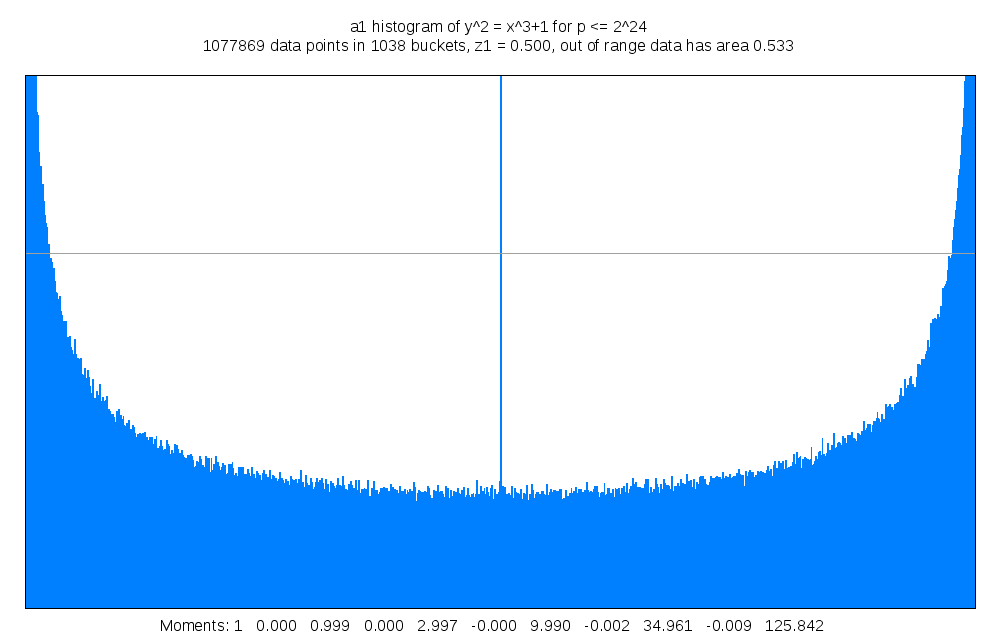
\includegraphics[scale=.3]{plots/Sato-Tate_CM.png}
\end{center}

The Sato-Tate conjecture is an analogous prediction for elliptic curves 
without complex multiplication. 

\begin{conjecture}[Sato-Tate]
Let $E$ be a non-CM elliptic curve over $\dQ$. Then the sequence 
$\{b_p(E)\}_p$ is equidistributed in $[-1,1]$ with respect to the 
measure 
\[
  \frac{2}{\pi} \sqrt{1-t^2}\, dt \text{.}
\]
\end{conjecture}

Here is the example $y^2=x^3+x+1$, also taken from Sutherland's web page. 

\begin{center}
  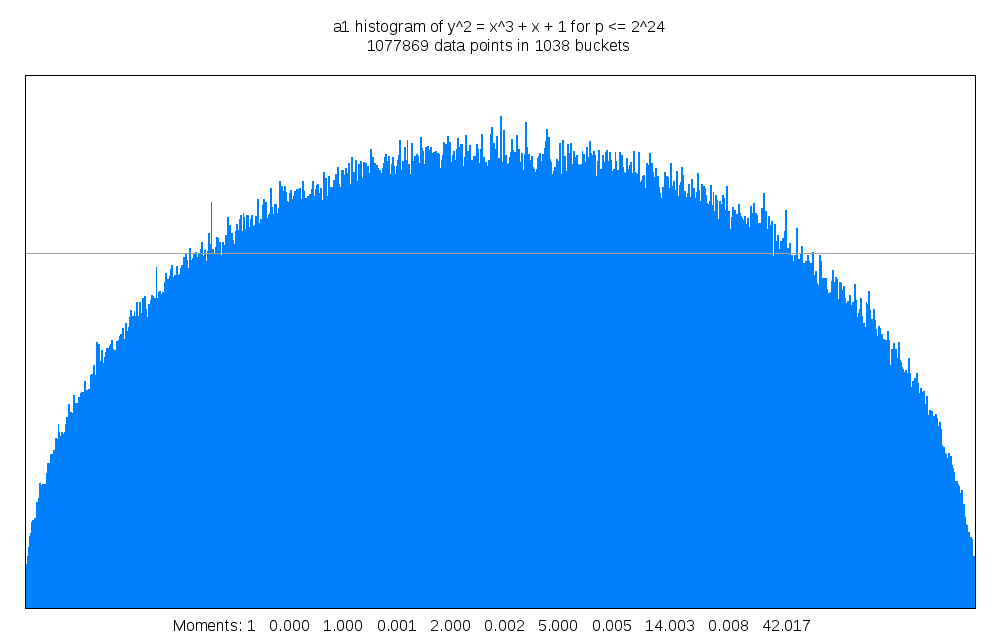
\includegraphics[scale=.3]{plots/Sato-Tate_nonCM.png}
\end{center}


\begin{theorem}[Barnet-Lamb, Geraghty, Harris, Taylor]
The Sato-Tate conjecture is true. 
\end{theorem}
\begin{proof}
See \cite[8.3]{bght09} for a (as yet unrefereed) proof. 
\end{proof}

There is a refined version of the Sato-Tate conjecture. Let 
$\rho=\{\rho_\ell:G_\dQ \to GL(2,\dZ_\ell)\}$ be a strictly compatible family 
of $\ell$-adic representations in the sense of \cite[ch.1]{se68}. For almost 
all primes $p$, the characteristic polynomial of $\rho_\ell(\frob_p)$ will be 
of the form $t^2 - a_p t + p$. Assume $\rho$ is \emph{pure} in the sense that 
the roots $\alpha_p,\bar\alpha_p$ of $t^2-a_p t+p$ are $q$-Weil. 

\begin{conjecture}[Lang-Trotter]
For any integer $n$ and imaginary quadratic field $k$, there are constants 
$C(n,\rho)$ and $C(k,\rho)$ such that 
\begin{align*}
  \#\{ p\leqslant x : \dQ(\alpha_p) = k\} &\sim C(k,\rho) \frac{\sqrt x}{\log x} \\
  \#\{p\leqslant x : a_p = n\} &\sim C(n,\rho) \frac{\sqrt x}{\log x} \text{.}
\end{align*}
\end{conjecture}

See the introduction to \cite{lt76} for the original statement and some 
motivation. 





% on 11-21-2013
\subsection{Some computations}

Let $d=157$. We hope to show that $d$ is congruent, i.e. that is is the area 
of a right triangle with rational side lengths. In other words, the curve 
$C_d$ defined as the solution set to 
\begin{align*}
  a^2+b^2 &= c^2 \\
  a b/2 &= d
\end{align*}
has a rational point. We have seen that this is equivalent to the elliptic 
curve $E_d:y^2=x^3-d^2 x$ having positive rank. 

We'll use Sage to do this. Sage can be accessed online at 
\url{http://sagenb.com/}, or just type \texttt{sage} in the command line of a 
computer that has Sage installed. 

In Sage, the constructor 
$\mathtt{EllipticCurve([}a_1,a_2,a_3,a_4,a_6\mathtt{])}$ returns the 
elliptic curve 
\[
  y^2 + a_1 x y + a_3 y = x^3 + a_2 x^2 + a_4 x + a_6 \text{.}
\]
The simpler constructor 
$\mathtt{EllipticCurve([}a_4,a_6\mathtt{])}$ returns the elliptic curve 
$y^2 = x^3+a_4 x + a_6$. Sage will return an error if the curve you try to 
construct is singular. Since we are interested in the curve 
$E_{157}:y^2=x^3-157^2 x$, we define 
\begin{sageblock}
E = EllipticCurve([-157^2, 0])
\end{sageblock}
If we had wanted to define an elliptic curve over a finite field $\dF_q$, we 
would make sure some of the coefficients were elements of $\dF_q$, as in 
\texttt{EllipticCurve([GF(5)(1), 1])}. We can compute the conductor of 
by \texttt{E.conductor()}; in our case $E_{157}$ has conductor 
$\sage{factor(E.conductor())}$. Usually one can compute the rank 
\texttt{E.rank()} and generators for the Mordell-Weil group 
\texttt{E.gens()}. In our case, these return a warning. Sage's usual algorithm 
was not able to determine the rank of $E_{157}$, and it asks you to do a 
two-descent. We do this: 
\begin{sageblock}
E.two_descent(second_limit=13)
\end{sageblock}
\begin{sagesilent}
P = E.gens()[0]
x,y = P[0], P[1]
pair = (abs((157^2-x^2)/y), abs(2*157*x/y))
\end{sagesilent}
As Sage does the $2$-descent, it outputs a bunch of text describing what it 
does (essentially a computation of $E(\dQ)/2$ and 
$\sha(E)[2]$). Once the $2$-descent is complete, we can compute the rank to be 
$\sage{E.rank()}$ and a generator to be 
\[
  \sage{P} \text{.}
\]
This corresponds to a triangle with the shorter two sides being 
\[
  \sage{pair} \text{.}
\]

There are a number of other things that Sage can do with elliptic curves. To 
make computations faster, let's try the elliptic curve 
\begin{sageblock}
E = EllipticCurve([4,6])
\end{sageblock}
described by the equation $\sage{E}$. This curve has rank $\sage{E.rank()}$ and 
generator $\sage{E.gens()[0]}$. We can do computations with points on our 
curve: 
\begin{sageblock}
P = E.gens()[0]
5*P # as an element of E(Q)
P.height() # Neron-Tate height of P
\end{sageblock}
A lot of analytic data can be computed: 
\begin{sageblock}
E.torsion_subgroup() # trivial for this curve 
L = E.lseries().dokchitser() # the L-function of E
L(1) # looks like zero
L.derivative(1,2) # non-zero, so r_an<=1
E.root_number() # sign in function equation (=-1, so r_an is odd) 
E.regulator() 
E.sha().an() # predicted order assuming BSD
\end{sageblock}

A fantastic place to learn more about Sage is its documentation page at 
\url{http://www.sagemath.org/doc/}. 






\subsection{The Sato-Tate conjecture and Haar measures}

Let $E$ be an elliptic curve over $\dQ$. Recall we defined 
$b_p(E) = a_p(E)/2\sqrt p$. If $E$ has CM, then the $b_p$ are 
uniformly distributed in $[-1,1]$ with respect to the measure 
\[
  \frac 1 2 \delta_0 + \frac{dt}{2\pi\sqrt{1-t^2}} \text{,}
\]
and if $E$ is not CM, then the $b_p$ are uniformly distributed with respect to 
\[
  \frac{2}{\pi} \sqrt{1-t^2}\, dt \text{.}
\]
This has a natural reformulation which makes generalization easier. The 
characteristic polynomial of $\rho_{E,\ell}(\frob_p)$ is 
$t^2-a_p t + p$. If we normalize to have roots with absolute value $1$, we get 
$\varphi_p = t^2 - \frac{a_p}{\sqrt p} t + 1$. This is the characteristic 
polynomial of a unique conjugacy class in $\operatorname{SU}(2)$. If we write 
$X$ for the space $\operatorname{SU}(2)^\natural$ of 
conjugacy classes in $\operatorname{SU}(2)$, then $p\mapsto \varphi_p$ can be 
thought of as a map $\{\text{primes}\} \to X$. Embed $\operatorname{U}(1)$ in 
$\operatorname{SU}(2)$ by the diagonal, and let $K=N(\operatorname{U}(1))$ be 
its normalizer. The group $K$ is compact, so it has a unique normalized Haar 
measure.

\begin{theorem}
If $E$ is an elliptic curve with complex multiplication, then the 
set $\{\varphi_p(E)\}\subset \operatorname{SU}(2)^\natural$ is 
equidistributed with respect to the pushforward of the normalized Haar measure 
on $N(\operatorname{U}(1))$. 
\end{theorem}
\begin{proof}
This is a restatement of Theorem \ref{thm:deuring-hecke}. To see this, note 
that the trace map induces an isomorphism 
\[\xymatrix{
  \trace : \operatorname{SU}(2)^\natural \ar[r]^-\sim 
    & [-2,2] \text{.}
}\]
The group $K=N(\operatorname{U}(1))$ has two connected components, both 
isomorphic to $S^1$:
\[
  K = 
  \left\{\begin{pmatrix} 
    z & \\ 
    & \bar z 
  \end{pmatrix} : |z|=1 \right\} 
  \cup \left\{\begin{pmatrix}
         & -z\\ 
         \bar z & 
       \end{pmatrix} : |z|=1\right\} \text{.}
\]
The first connected component is mapped to $[-2,2]$ via 
$z\mapsto 2\Re (z)$, and the second is mapped via $z\mapsto 0$. It is easy to 
check that the pushforward of the Haar measure on $K$ is exactly 
$\frac 1 2 \delta_0 + \frac{dt}{2\pi \sqrt{4-t^2}}$. 
\end{proof}

For non-CM elliptic curves, let $K=\operatorname{SU}(2)$. Then the Sato-Tate 
conjecture states that $\{\varphi_p\}\subset \gl{2}{\dC}^\natural$ is 
uniformly distributed with respect to the pushforward of the normalized Haar 
measure on $K$. To see this, check that the pushforward by the trace of the 
normalized Haar measure on $K$ to $[-2,2]$ is $\frac{1}{2\pi} \sqrt{4-t^2} dt$. 

More generally, let $A$ be a $d$-dimensional abelian variety over $\dQ$, and 
let $\ell$ be a prime at which $A$ has good reduction. For any prime $p$ of 
good reduction, we have the characteristic polynomial $P_{A_p}$ of the 
Frobenius at $p$ acting on $T_\ell A$. The roots of this polynomial are 
$p$-Weil, so if we write $P_{A_p}(t) = \prod (t-\omega_i)$, then the polynomial 
$\varphi_p(A) = \prod \left(t-\frac{\omega_i}{\sqrt p}\right)$, has roots with 
absolute value $1$. Then by \cite[13.1]{ka88}, $\varphi_p(A)$ determines a 
conjugacy class in $\operatorname{SU}(2 d,\dC)$. As before, we think of 
$\varphi(A)$ as a map 
$\{\text{good primes}\}\to \operatorname{GL}(2 d,\dC)^\natural$. 

\begin{conjecture}[Serre]
There exists a compact real Lie group $K$ in $\gl{2d}{\dC}$ such 
that $\{\varphi_p(A)\}\subset \gl{2d}{\dC}^\natural$ is equidistributed with 
respect to the pushforward of the normalized Haar measure on $K$. 
\end{conjecture}

There is a conjectural prediction of the group $K$, which we will treat in the 
next section. 





\subsection{Motives and the refined Sato-Tate conjecture}

The following mostly follows Serre's original paper \cite{se94}, but see 
\cite{se12} for a more elementary and explicit approach. 

Let $k$ be a field, and let $X$ be an $n$-dimensional smooth variety over $k$. Write 
$\chow(X) = \chow^\bullet(X)$ for the Chow ring of $X$, consisting of algebraic 
cycles modulo rational equivalence. The intersection product makes $\chow(X)$ 
into a commutative unital ring -- for details, see \cite[8.3]{fu98}. There is a 
natural ``composition'' map 
\begin{equation*}\tag{$*$}\label{eq:compose-cycles}
  \chow(Y\times Z)\otimes \chow(X\times Y) \to \chow(X\times Z) \text{,}
\]
defined by 
$g\circ f = \pi_{X\times Z, \ast}(\pi_{Y\times Z}^\ast g\cdot \pi_{X\times Y}^\ast f)$. 
This satisfies all of the natural linearity and functoriality properties one 
would expect \cite[16.1]{fu98}. 

There is a canonical ``degree map'' $\deg:\chow^n \to \dZ$, and we say a cycle 
$\alpha \in \chow^r(X)$ is \emph{numerically equivalent to zero} if 
$\deg(\alpha\cdot \beta)=0$ for all $\beta\in \chow^{n-r}(X)$. Write 
$\chow_\text{num}(X)$ for the quotient of $\chow(X)$ by the (graded) ideal 
generated by 
\[
  \{\alpha\in \chow(X) : \alpha\text{ is numerically equivalent to zero}\} \text{.}
\]

\begin{definition}
Let $k$ be a field. A \emph{(pure) motive over $k$} is a triple 
$(X,e,r)$, where $X$ is a smooth projective variety over $k$, 
$e\in \chow_\textnormal{num}(X\times X)_\dQ$ is an idempotent, and 
$r\in \dZ$. 
\end{definition}

See \cite[4.1.3]{an04} for details. One defines a morphism 
$(X,e,r) \to (Y,f,s)$ to be an element of 
\[
  f\cdot \chow^{\dim X - r - s}(X\times Y)_\dQ\cdot e \text{.}
\]
Morphisms are composed via the ``composition map'' \eqref{eq:compose-cycles}. 

With this, write $\motives(k)$ for the category of (numerical) motives over 
$k$. Let $\mathsf{SmProj}_k$ be the category of smooth projective varieties 
over $k$, and let $h:\mathsf{SmProj}_k \to \motives(k)$ be the functor 
$X\mapsto (X,\Delta_X,0)$. The category $\motives(k)$ is obviously $\dQ$-linear, and 
has a Tannakian structure induced by $h(X)\otimes h(Y) = h(X\times Y)$. In 
fact, $\motives(k)$ is a semisimple abelian category \cite{ja92}. One should 
think of a Weil cohomology theory as a functor 
$\h:\motives(k) \to \mathsf{grAlg}_L$ for some field $L$ (c.f. 
\cite[4.2.5.1]{an04}). 

Write $1=\h(\dA^0)$ for the trivial motive. Since every variety has a unique 
morphism $X\to \dA^0$, there is a unique morphism $1\to M$ for every motive 
$M$. The rational point $\infty\in \dP^1$ determines a splitting of 
$1\to h(\dP^1)$, hence a direct sum decomposition $h(\dP^1)=1\oplus 1(-1)$, 
where $1(-1)$ is the motive $(\dP^1,[\infty]\times \dP^1,0)$. We define 
$1(r)=1(-1)^{\otimes(-r)}$; these are called \emph{Tate motives}. In general, 
put $M(r) = M\otimes 1(r)$. There is a decomposition 
$h(\dP^n) = 1\oplus \cdots \oplus 1(-n)$. If $A$ is a $d$-dimensional abelian 
variety over $k$, then there is a unique decomposition 
$h(A)=h^0(A)\oplus \cdots \oplus h^{2 d}(A)$ in $\motives(k)$ such that 
$[n]$ acts as multiplication by $n^i$ on each $h^i(A)$ \cite[13.29]{gm13}. %\cite[3.1]{ku94}. 
What is more, there are canonical isomorphisms 
$h^i(A)\simeq \bigwedge^i h^1(A)$, inducing an isomorphism 
$h(A)\simeq \bigwedge^\bullet h^1(A)$ (13.47, loc. cit.). 


Let $k$ be a number field, and choose an embedding 
$\sigma:k \hookrightarrow\dC$. We have a Betti realization functor 
$\h_\sigma:\motives(k) \to \mathsf{grAlg}_\dQ$, assigning to a motive 
$M = (X,e,r)$ the vector space 
\[
  \h_\sigma(M) = e^\ast \cdot \h_\text{sing}^\bullet(X(\dC), \dQ) \otimes \h^2(\dP^1)^{\otimes (-r)}
\]
Assuming Grothendieck's standard conjectures, the functor $\h_\sigma$ is a 
\emph{fiber functor}, so $\mathsf{M}(k)$ is equivalent to the category of 
representations of the (pro-reductive) \emph{motivic Galois group} 
\[
  G_\text{mot}(k) = \aut^\otimes(\h_\sigma) = \left\{(x_M)\in \prod_{M\in\motives(k)} \operatorname{GL}(\h_\sigma M) : x_M\circ f^\ast = f^\ast\circ x_N\text{ for }f:M\to N \right\}\text{.}
\]
For a motive $M$, let $G_M$ be the automorphism group of the restriction of the 
fiber functor to the largest Tannakian subcategory of $\motives(k)$ containing 
$M$. There are obvious projections from $G_\text{mot}(k)$ to the groups $G_M$. 

Let $M$ be a motive. There is a map $w:\dG_m \to G_M$, induced by the grading 
$\h_\sigma M = \bigoplus \h_\sigma^d(M)$. The action of $a\in \dG_M$ on the 
$d$-th piece is by $a^{-d}$. For example, if $E$ is an elliptic curve without 
complex multiplication, then for $M=h^1(E)$, $G_M=\operatorname{GL}(2)$ and 
$w:\dG_m \to \operatorname{GL}(2)$ is the inverse of the canonical injection. 

For a motive $M$, there are $\ell$-adic realizations $\h_\ell(M)$ coming from 
\'etale cohomology. After we fix a prime $\ell$, the representation 
$\rho_{M,\ell}$ is unramified at all but finitely many places. For those 
unramified places $v$, put 
$\varphi_v(M) = w(N v^{1/2}) \rho_{M,\ell}(\frob_v)$. 

Let $T=1(-1)$ be the Tate motive, and let $t:G_\text{mot}(k) \to G_T$ be the 
canonical projection. For any motive $M$, let $G_M^1$ be the image of 
$\ker(t)$ under the projection $G_\text{mot}(k) \to G_M$. 

\begin{conjecture}[Serre]
Let $M$ be a motive over a number field $k$. Let $K$ be a maximal compact 
subgroup of $G_M^1$. The elements $\varphi_v(M)$ have eigenvalues in 
$\bar\dQ$, and determine a unique conjugacy class (independent of $\ell$) 
$\varphi_v(M) \in G_M^1(\dC)^\natural$. The set 
$\{\varphi_v(M)\}\subset G_M^1(\dC)^\natural$ is equidistributed with respect 
to the pushforward of the normalized Haar measure on $K$. 
\end{conjecture}






\subsection{The Bloch-Kato conjecture}

Let $E$ be an elliptic curve over $\dQ$. Recall that the (strong) Birch and 
Swinnerton-Dyer conjecture is the formula 
\[
  \lim_{s \to 1} \frac{L(E,s)}{(s-1)^{\rank E}} = \frac{\Omega_E \regulator_E \# \sha(E) \prod_p c_p}{\# E(\dQ)_\text{tors}^2} \text{,}
\]
together with the claim that everything involved is well-defined and finite. 
For a number field $k$, recall that the \emph{Dedekind zeta function} of $k$ 
is the series 
\[
  \zeta_k(s) = \sum_{\fa\subset \fo_k} \frac{1}{(N\fa)^s} \text{,}
\]
where $N\fa = [\fo_k:\fa]$ for an ideal $\fa$. It is a theorem that $\zeta_k$ 
has an analytic continuation to $\dC\smallsetminus 1$. The pole at $s=1$, and 
we have the following analytic \emph{class number formula}. Let $r$ be the 
order of the pole of $\zeta_k$ at $1$, and let $r_1,r_2$ be the number of 
real (resp. complex) places of $k$. Let $h_k$ be the class number of $k$, $d_k$ 
be the discriminant of $k$. Then 
\[
  \lim_{s \to 1} \frac{\zeta_k(s)}{(s-1)^r} = \frac{2^{r_1} (2\pi)^{r_2}|d_k|^{-1/2} \regulator_k h_k}{\# \mu(k)} \text{.}
\]

The Birch and Swinnerton-Dyer conjecture as well as the class number formula 
are both special cases of a very far-reaching generalization called the 
\emph{Bloch-Kato conjecture}. 

\textbf{(add BSD for abelian varieties, brief statement of Bloch-Kato)}





